\chapter{Data Management experiment} 
\label{cha:transf}

In this appendix we present the experiment that we performed in order to evaluate the qualities of the Data Management solution. In order to do that, we took an already existing user modelling service, implemented it using the newly proposed solution and at the end, discuss the improvements. 

For the experiment we used the already implemented service for building language profiles based on Twitter. The basic idea of the workflow is to read all tweets for a particular user form the database, infer the languages (and level of knowledge) that the user knows, store the generated profile in the database and finally, provide it as a result of the execution of the service.

\begin{figure}[h!]
  \centering
  	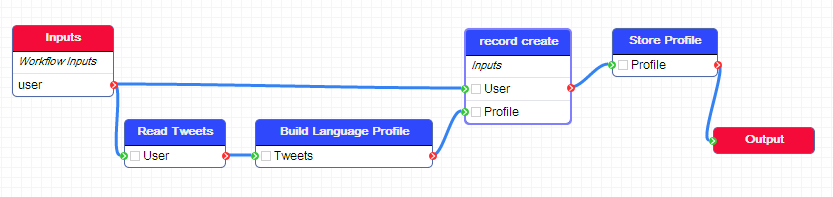
\includegraphics[scale=0.65]{storage/eval/before.png}
  \caption{Workflow defining the service for building language profiles before the introduction of the feature}
  \label{fig:storageEvalBefore}
\end{figure}

Figure \ref{fig:storageEvalBefore} shows how the workflow looked like before the introduction of our solution. In order to implement that workflow engineers had to perform the following steps:
\begin{itemize}
	\item Install and set-up a database.
	\item Create the necessary tables manually. This step is required every time the workflow is deployed on a U-Sem system. 
	\item Implement specific components for queering the tweets and storing the generated profiles and deploy them to the U-Sem system.
	\item Make the store component return a copy of its input because it has to be part of the main branch otherwise it is optimized by the engine and not executed.
\end{itemize}

\begin{figure}[h!]
  \centering
  	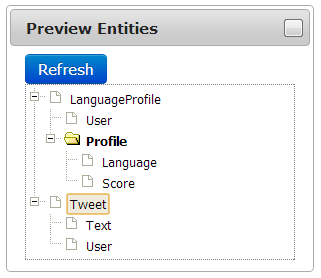
\includegraphics[scale=0.65]{storage/eval/entities.png}
  \caption{The entity definitions needed for building the service for building language profiles}
  \label{fig:storageEvalEntities}
\end{figure}

Figure \ref{fig:storageEvalAfter} shows how the workflow looks like after the introduction of our solution. In order to implement the workflow engineers had to perform the following steps:
\begin{itemize}
	\item Define the entity types using the user interface illustrated on Figure \ref{fig:storageEvalEntities}.
	\item Reuse the components for querying and storing data by only providing the required JPQL query and selecting the entity type for storing.
	\item Indicate the store component to have side effects and put it in a separate branch.
	\item Pack the workflow and entity types definitions into a plug-in for easy deployment.
\end{itemize}

\begin{figure}[h!]
  \centering
  	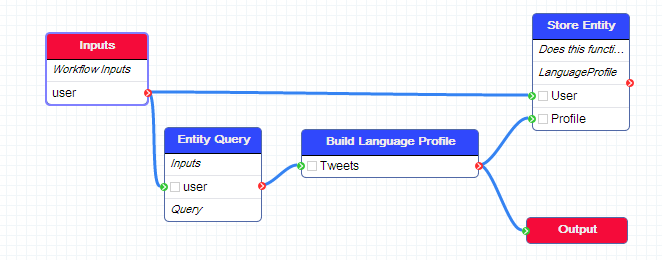
\includegraphics[scale=0.65]{storage/eval/after.png}
  \caption{Workflow defining the service for building language profiles after the introduction of the feature}
  \label{fig:storageEvalAfter}
\end{figure}

We can conclude that using the proposed solution provided the following advantages compared to the initial situation:

\begin{itemize}
	\item No installation and configuration of a database is required.
	\item No need to create the database schema manually. It is done automatically by the user interface.
	\item No programming required for implementing storage and query components.
	\item No need to convert RGL values so that they can fit into the database.
	\item Queries are written in JPQL which is a higher level language compared to SQL and queries were faster and easier to write. Additionally, the user interface that shows the structure of the entities at any time makes writing queries easier (engineers do not have to know it by heart) and prevents mistakes that come from not knowing the structure of the entities. 
	\item The workflow looks more intuitive because the storage component can be left in a separate branch and does not have to return a copy of the input data like in the initial situation.
	\item The workflow can be deployed on a U-Sem system by simply installing the plug-in. No configuration required.
\end{itemize}
